\documentclass[bare_jrnl_transmag]{subfiles}
\begin{document}
\subsection{Kalman Filter Theory}
A Kalman Filter is a type of algorithm which predicts the states of a system using their dynamics, and correcting the prediction with feedback from an external sensor. The filter is used to fuse the data coming from the IMU and the data from the camera. 
In the case of the project, the Kalman filter was used to predict the position of the drone relative to the world frame. The states of the Kalman Filter were thus 

\begin{equation} 
    [ t_x, t_y, t_z, v_x, v_y, v_z ] 
\end{equation}  which represent the translation and velocity of the drone in world frame. 
The inputs of the system will be the IMU acceleration data and the camera distance output, while the output of the system will be the updated position of the drone.

The filter uses various noise and covariance matrices to add uncertainty to the model. THe main matrices are the P, Q and R matrix. The P matrix - State Covariance Matrix, is responsible for representing the uncertainty in the system states. It essentially represents the trust in the state variables vs the measured values.
The Q and R matrix represent two diffeent noise matrices. The Q matrix represents the process noise matrix, which models the uncertainty in the system dynamics. If simplifications are made, or affects ignored, this term helps account for that variation. The R matrix represents the Measurement Noise, which models how noisy the sensor measurement truly is. 

Together these matrices, along with the calculated outputs from the predict and measurment stage are used to calculate the Kalman Gain. This gain weighs the prediction vs the measured state to create the required output. 

\subsubsection{Predict}
The predict stage of the Kalman Filter is responsible for taking in the system inputs and determining the new states based on the dynamics of the system. In the case of the drone, the assumption of linear displacement was made due to the quick sampling time of the IMU. The dyanmics of the drone flight is based on linear motion laws. Since the input of the predict step is the acceleration of the drone in the drone frame, a couple modifications must be made to the data. Firstly, the linear acceleration must be integrated to get distance. The data is presented in a time series format, which means that a discritezed integration is required. For this system, instead of directly integrating the acceleration for displacement, the previous velocity is integrated to determine the change in distance and then the new acceleration is integrated to determine the new velocity. Since the time steps are so small, it can be assumed that the velocity will not change largely between the time steps. 
Before processing the acceleration in world frame, the acceleration from the IMU (in IMU/Drone frame) needs to be rotated towards the current pose. An assumption that the pose does not change much during the time step is made to remove the circular dependancy. To convert the acceleration from drone frame to world frame, the pose from the madwick filter is fed into a combined rotation matrix. This matrix is applied to the acceleration to get the accleration in the world xyz frame.

Once the world frame acceleration is calculated, the position and velocity states of drone can be computed.

The equations look as follows:


\begin{align*}
    \textbf{Velocity:} \\
    v_x[k] &= v_x[k-1] + a_x[k] \cdot \Delta T \\
    v_y[k] &= v_y[k-1] + a_y[k] \cdot \Delta T \\
    v_z[k] &= v_z[k-1] + a_z[k] \cdot \Delta T
    \end{align*}
    
    \begin{align*}
    \textbf{Displacement:} \\
    t_x[k] &= t_x[k-1] + v_x[k] \cdot \Delta T \\
    t_y[k] &= t_y[k-1] + v_y[k] \cdot \Delta T \\
    t_z[k] &= t_z[k-1] + v_z[k] \cdot \Delta T
\end{align*}
    
As a state-space representation, the dynamics of the system can be written as follows:

\begin{align*}
    x[k] &= {\null\hbox{$\begin{bmatrix}
    t_x \\
    t_y \\
    t_z \\
    v_x \\
    v_y \\
    v_z
    \end{bmatrix}$}}
    \quad
    u[k] = {\null\hbox{$\begin{bmatrix}
    a_x \\
    a_y \\
    a_z
    \end{bmatrix}$}}
\end{align*}

\begin{align*}
    A &= 
    \begin{bmatrix}
    1 & 0 & 0 & \Delta T & 0 & 0 \\
    0 & 1 & 0 & 0 & \Delta T & 0 \\
    0 & 0 & 1 & 0 & 0 & \Delta T \\
    0 & 0 & 0 & 1 & 0 & 0 \\
    0 & 0 & 0 & 0 & 1 & 0 \\
    0 & 0 & 0 & 0 & 0 & 1 \\
    \end{bmatrix}
    \\[1em]
    B &=
    \begin{bmatrix}
    0 & 0 & 0 \\
    0 & 0 & 0 \\
    0 & 0 & 0 \\
    \Delta T & 0 & 0 \\
    0 & \Delta T & 0 \\
    0 & 0 & \Delta T \\
    \end{bmatrix}
    \\[1em]
    x[k+1] &= A \cdot x[k] + B \cdot u[k]
    \\[1em]
    C &=
    \begin{bmatrix}
    1 & 0 & 0 & 0 & 0 & 0 \\
    0 & 1 & 0 & 0 & 0 & 0 \\
    0 & 0 & 1 & 0 & 0 & 0 \\
    \end{bmatrix}
\end{align*}


The predicted uncertainty of the states are also recomputed at the end of the predict state suing the following equation.

\begin{equation*}
    P_{k|k-1} = A * P_{k-1|k-1} A^T + Q
\end{equation*}


    
\subsubsection{Update}
The Update phase of the Kalman Filter is where the sensor fusion occurs. In essence, the predicted state is compared to another state (i.e. the camera output) to fuse the data together. 
The Kalman Gain, or K Matrix, determines the weight of the predicted state vs the model state. It is calculated using the error covariance matrix, the measurement noise matrix and the output state matrix. 
At each update step, the matrix is updated for the new gain, essentially recording which state should be trusted more, model or actual.

The states are then updated using the Kalman Gain and the outputs of the camera and prediction.

\begin{eqnarray*}
    K_k = P_{k|k-1} C^T * (C P_{k|k-1} C^T + R)^{-1} \\
    P_{k|k} = (I - K_k C) P_{k|k-1}
\end{eqnarray*}

The estimate is also updated using the states from the predict step and the states of the sensor, in our case being the camera. 
The estimated measurements are denoted with $\hat{x}$, whereas the sensor measurements are denoted regularly. 
\begin{equation*}
    \hat{x}_{k|k} = \hat{x}_{k|k-1} + K_k (z_k - H \hat{x}_{k|k-1})
\end{equation*}

\subsubsection{Implementation}

The Kalman Filter was implemented in Python by developing a class which encapsulated the predict and update steps. 

The class, named ImuKalmanFilter, was designed to be used with the IMU and camera data. The class is instantiated with initial state, dt, initial covariance, process noise, measurement noise, the number of states, and the gyro bias. 

The class consists of two functions -- update, and predict. 

The update function takes the output of the Madgwick filter - the acceleration and angular velocities in drone frame. These are then converted to world frame using rotation matrices Using the previous state velocities, the current position of the drone in the world frame is updated. Furthermore, the velocities are also updated using the most recent acceleration data. Finally, the covariance matrix, P is updated in the predict step.

The predict function takes the camera data and the current state of the drone. The camera data is used to update the Kalman Gain, which is then used to update the state of the drone. The covariance matrix is also updated in this step.

The linear algebra operations and definition of the matrices are done using the Numpy library. The rotation matrices are defined using the Euler angles from the Madgwick filter. 

\subsection{Performance}
The performance of the Kalman Filter was validated by plotting the output of the filter against the ground truth position of the drone in the world frame. The ground truth position was parsed from the dataset, and the Kalman Filter was run on the raw sensor data, also parsed from the dataset. Using Matplotlib, both of these results were plotted on a 3D graph, with the x, y and z axes representing the world frame. The Kalman Filter output was plotted in orange, while the ground truth was plotted in blue. 

\begin{figure}[H]
    \centering
    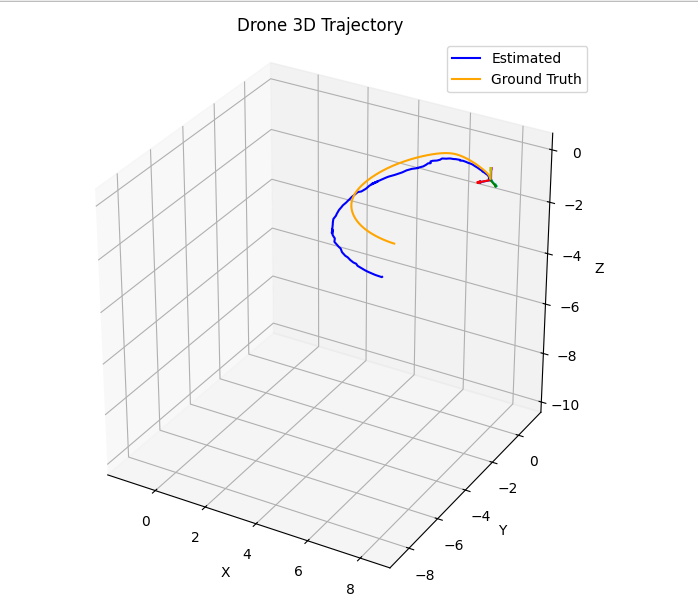
\includegraphics[width=0.8\linewidth]{figures/ekf_results.png}
    \caption{Kalman Filter results. The blue line is the ground-truth pose of the drone, while the orange line is the pose angle estimated by the Kalman filter.}
    \label{fig:kalman_results}
\end{figure}

It is observed that although the ground truth is tracked very well by the filter, there is observed drift, particularly on the z-axis. The Kalman Filter was tuned using the process and measurement noise matrices, which were iterated upon with different values to find the best fit. 

\end{document}